\begin{savequote}[8cm]
\textlatin{Neque porro quisquam est qui dolorem ipsum quia dolor sit amet, consectetur, adipisci velit...}

There is no one who loves pain itself, who seeks after it and wants to have it, simply because it is pain...
  \qauthor{--- Cicero's \textit{de Finibus Bonorum et Malorum}}
\end{savequote}

\chapter{\label{ch:1-intro}Introduction} 

\minitoc

\section{A plan}
Actually the very first thing to say will be the stuff about light i think, about diagnostic tools essentially always being about controlling the various properties of light (ie electromagnetic waves)

sections to include
start with the laser and our entrance into the multi-petawatt regime with no signs of stopping - ref 40 in alex savin thesis - it looks like that is saying huge growth in laser power check that and maybe write in thesis but don't include the figure. Also include description of CPA and OPCPA
what is a plasma
modelling plasma with PIC codes
intense lasers and absorption mechanisms?? yes for sure but dont do all just those just below ZVP
simulation units and similarity parameter
Frames of reference - lab, sim, ablating front sruface of plasma

what is the story? Based on first section by Alex after the abstract
Plasma is ubiquitous in our known universe and plasma provides us huge opportunities as a tool to improve our lives
(From chen) what we can see in the sky is a result of that stuff being in the plasma state.
Lasers can do so much now and are only getting more powerful all the time thanks to CPA and since developments (discuss)
Simulataneously our ability to understand the physics has been aided by an explosion in computing power (peter HEDP paper)
In this thesis we discuss some of the opportunities that relativistic laser plasma physics offers us with solid density targets - note that note about solids v gases at this point. 
Perhaps even before the debye length, define what we mean by the temperature of the plasma??

An unused statement about ion immobility
Assume for now that the ion-electron mass ratio is infinite, that is to say the ions are approximately immobile for the timescales under consideration, generally true for a fair few relativistic laser pulse cycles (In later sections the mobility of plasma ions will prove very important but for now this is ignored.).

\section{\label{sec:plasma_def}The definition of a plasma}
As outlined in F. Chen's definitive textbook `Introduction to Plasma Physics and Controlled Fusion' \cite{chen20116}, a plasma must fulfil three criteria, namely,

\begin{enumerate}
	\item Ionisation: a plasma must consist of both charged and neutral particles, of course this alone cannot define a plasma, any gas will contain some degree of ionisation;
	\item Quasineutrality: while locally there can be (often extreme) electromagnetic forces and charge concentrations at work, over the length scales of the plasma, such forces are screened out and the plasma bulk remains net neutral in charge;
	\item Collective behaviour: unlike in a gas where collisions dominate, the particles in a plasma generate electromagnetic fields that interact at a distance and thus a particle's motion depends not only on its immediate viscinity but on the surrounding plasma conditions, indeed often it is the so-called `collisionless' plasmas where collisions can be safely neglected that are of most interest, as is the focus of this thesis.
\end{enumerate}

\subsection{\label{sec:debye_length}The Debye length}
The Debye length describes the extent to which a plasma can shield electromagnetic fields within and so remain quasineutral. Consider an infinitely extending plasma with a test charge placed at some point, then what would be the potential $\phi(\mathbf{x})$? If the plasma had no kinetic energy, the charged particles would arrange themself immediately ajacent to the test charge and once this equilibrium state was reached there would be no electromagnetic fields present. Realistically the plasma will have some temperature, likely a very large temperature and so some particles will be able to escape the potential of the test charge and thus leak electromagnetic fields into the plasma bulk. Poisson's equation reads
\begin{equation}\label{eq:poisson}
	\epsilon_0\nabla^2\phi = -e(Zn_i - n_e),
\end{equation}
where $\epsilon_0 = \qty{8.854e-12}{F.m^{-1}}$ is the permittivity of free space, $e = \qty{1.602e-19}{C}$ is the charge of an electron, $Z$ is the plasma ion charge in units of $e$ and $n_i$ and $n_e$ are the number densities of plasma ions and electrons.

Since the electrons are significantly more mobile than the ions due to their lower mass, it is in general the electrons and not the ions that respond to the test charge and the ions can be assumed to provide a constant background of positive charge density.
If the number density of electrons follows a Boltzmann temperature distribution in the presence of a potential energy $-e\phi$, then
\begin{equation}\label{eq:nj_boltzmann}
	n_e= n_{e,0}e^{e\phi/KT_e},
\end{equation}
where $n_{e,0}$ is the electron number density far from the test charge, $n_i = n_{e,0}/Z$ and $KT_e$ is the electron temperature. Note that in plasmas it is very common for different species to have differing temperatures depending on the mechanism for energy absorption and the timescales for collisions compared to the timescale of the study.

Substituting equation \ref{eq:nj_boltzmann} into equation \ref{eq:poisson} and Taylor expanding the exponential term in the limit that the plasma is weakly coupled ($e\phi << KT_e$), obtains 
\begin{equation}\label{eq:poisson_debye2}
	\nabla^2\phi = \frac{\phi}{\lambda_D^2},
\end{equation}
where
\begin{equation}\label{eq:debye}
	\lambda_D \equiv \sqrt{\frac{\epsilon_0KT_e}{n_ee^2}},
\end{equation}
is the \textit{Debye length} and describes the thickness of the charge sheath surrounding the test charge. For quasineutrality to hold for the plasma bulk, its spatial dimensions must extend beyond a few Debye lengths.

\subsection{\label{sec:plasma_parameter}The plasma parameter}
In order for the above description to be statistically valid, there must be a large number of charged particles within the shielding sheath. The number of particles within the \text{Debye sphere} can be computed as
\begin{equation}\label{eq:plasma_parameter}
	N_D = \frac{4}{3}\pi\lambda_D^3n.
\end{equation}
Note that, as discussed above, in most cases it is most suitable to choose the number density $n$ to be the number density of electrons. To ensure the plasma is suitably ionised (criterion 1) and that the plasma engages in collective behaviour (criterion 3),
\begin{equation}\label{eq:plasma_parameter_condition}
	N_D >>> 1.
\end{equation}
\subsection{\label{sec:plasma_frequency}Collisionality and the plasma frequency}
Collective behaviour not only depends on the ability for large numbers of particles to interact via electromagnetic forces but that these forces dominate over collisions in describing particle trajectories. Taking $\omega$ as the typical frequency of plasma oscillations and $\tau$ as the average time between collisions, for a plasma (as opposed to a gas) must satisfy
\begin{equation}\label{eq:plasma_frequency_condition}
	\omega\tau > 1.
\end{equation}
It now remains to determine what is the typical frequency of collisions in a given plasma. While the types of plasma waves and their associated frequencies of oscillation are multitudinous, the characteristic frequency, the \textit{plasma frequency}, $\omega_p$, is the most straightforward. It describes the response of electrons to charge imbalances within an infinite uniform plasma at rest in the absence of magnetic fields or temperature fluctuations. As noted in section \ref{sec:debye_length}, the ions provide a constant backgorund of positive charge.

Consider an semi-infinite plasma existing for $x>0$, with electron density $n_e$ and ion density $n_e/Z$ of charge state $Z$\footnote{This description has direct relevance to the Zero Vector Potential mechanism which will be made clear later.}. Suppose the electron fluid is displaced by some perfectly isotropic force into the plasma bulk a distance $(\Delta x) \hat{\mathbf{x}}$ as in figure \ref{fig:introplasmafrequency}. 
\begin{figure}
	\centering
	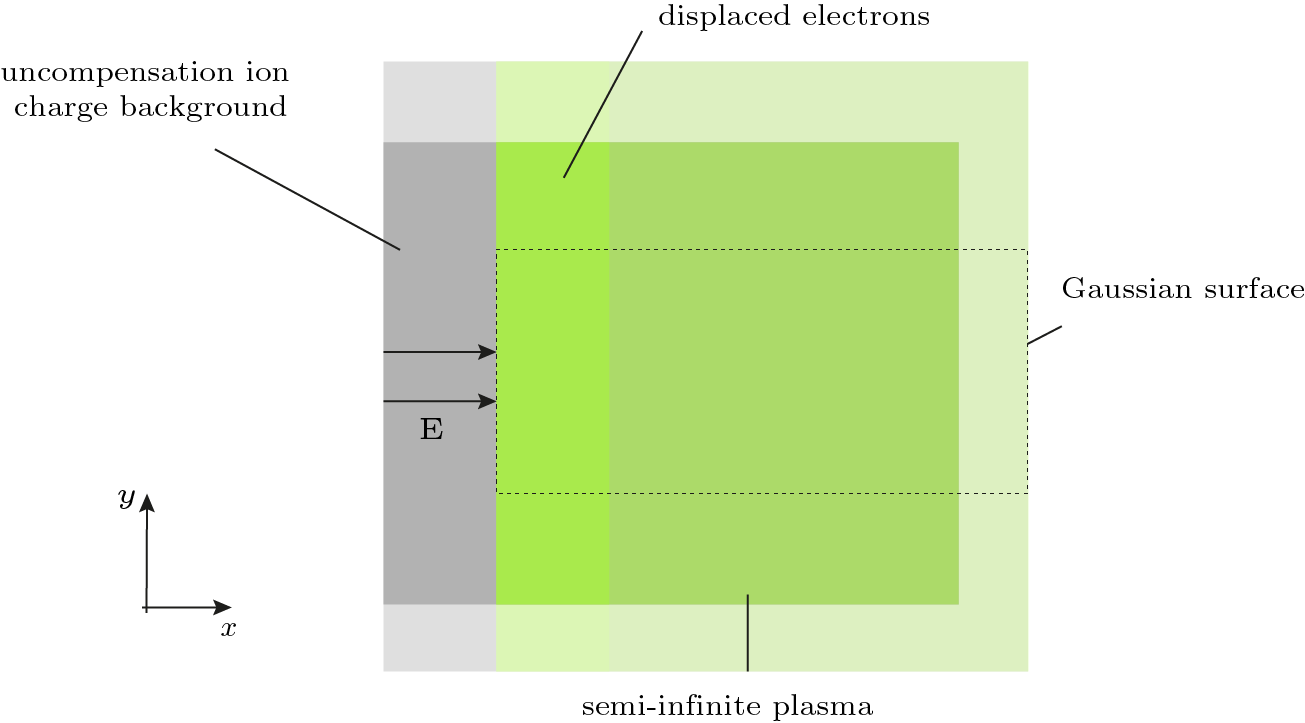
\includegraphics[width=0.7\linewidth]{figures/intro/intro_plasma_frequency}
	\caption{Diagram to illustrate the plasma frequency derivation.THIS FIGURE NEEDS E POINTING THE OTHER WAY}
	\label{fig:introplasmafrequency}
\end{figure}
The total charge of displaced electrons within a surface area of $\sigma$ is 
\begin{equation}\label{eq:intro_Q}
	Q = -en_\mathrm{e}\sigma\Delta x.
\end{equation}
Applying Gauss' law to the surface detailed in figure \ref{fig:introplasmafrequency}, the uncompensated charge leads to 
\begin{equation}\label{eq:intro_E}
	-\sigma E\hat{\mathbf{x}}= \frac{Q}{\epsilon_0}\hat{\mathbf{x}} = -\frac{en_e\sigma\Delta x}{\epsilon_0}\hat{\mathbf{x}}
\end{equation}
at the electron surface. By the Lorentz force, the displaced electrons will experience a restoring force, $-eE\hat{\mathbf{x}}$, perpendicular to the surface due to the electron-ion charge imbalance. The equation of motion for electrons on that surface is therefore
\begin{equation}\label{eq:intro_sho}
	m_e\frac{\mathrm{d}^2\Delta x}{\mathrm{d}t^2} = -eE = -\frac{e^2n_e}{\epsilon_0}\Delta x.
\end{equation}
Equation \ref{eq:intro_sho} clearly describes a simple harmonic oscillator with a characteristic frequency given by the plasma frequency,
\begin{equation}
	\omega_p = \sqrt{\frac{e^2n_e}{m_e \epsilon_0}}.
\end{equation}



\section{The Lawson-Woodward theorem}\label{sec:intro-lawson_woodward}
The Lawson-Woodward theorem states that there can be no net electron energy gain using laser fields \cite{esarey_2009_PhysicsLaserdrivenPlasmabaseda}, quite at odds with one of the primary aims of this thesis, that is, the acceleration of electrons. There are, however, several conditions that must be met, namely,
\begin{enumerate}
	\item The interaction region is infinite;
	\item The interaction  occurs in a vacuum;
	\item The electron is ultra-relativistic ($v\approx c$) along the acceleration gradient;
	\item No electro- or magnetostatic fields are present;
	\item Non-linear effects are neglected.
\end{enumerate}
Several of these will be applicable to the various accelerations of electrons considered. It is this final condition that is most damning, throughout this thesis the ultra-relativistic laser pulses under consideration ensure non-linear effects cannot be neglected. It is indeed such non-linearities that are of interest.


